\documentclass[uplatex]{jsreport}
\usepackage{docmute}
\usepackage{myStyle}
\label{chapterXX}

\begin{document}

\chapter{要因計画と平均値差の検定}
ここまでは主に，平均値の比較に確率的判断の手続きを加えた仮説検定の話をしてきました。
ここでは前期の最後に学んだ，線形モデルから要因計画へと進んだ話に，検定の話を統合します。線形モデルに確率的判断の手続きを加えたものが，分散分析と呼ばれる独自の体系になります。ここでは線形モデルの一環であることを意識しつつ，質的説明変数によって水準同士の対比較になることによる分析の手順について理解することを目的とします。水準が多くなった場合の対比較には，検定の多重性の問題が影響してくるため，問題を回避するために多重比較と言う考え方も導入する必要があります。

\section{平均値の比較とモデル比較}
前期の話の流れを思い出すと，わからないことをモデルで考え(第\ref{chapter5},\ref{chapter6},\ref{chapter7}講)，関係性を線形モデルで表現し(第\ref{chapter8},\ref{chapter9}講)，その特殊例として実験計画法がある(第\ref{chapter11}講)，という流れでした。

後期に入ってから，確率の使い方が母集団を対象にしたものに変わりました。これまでは誤差が正規分布するから，という理由で確率が導入されていましたが，様々な誤差に影響された誤差まみれの数字は，正規分布するという正規分布の別の側面からアプローチしてきたのです。また，母集団と標本という区別をおくことで，母集団の分布についての仮定から，標本統計量の分布が考えられ，それを使って母数を推測するという方法を取りました。母数を推測するだけでなく，実践的な判断をする帰無仮説検定という手続きについても，解説してきました。

\begin{wrapfigure}{r}{8cm}
    \centering
    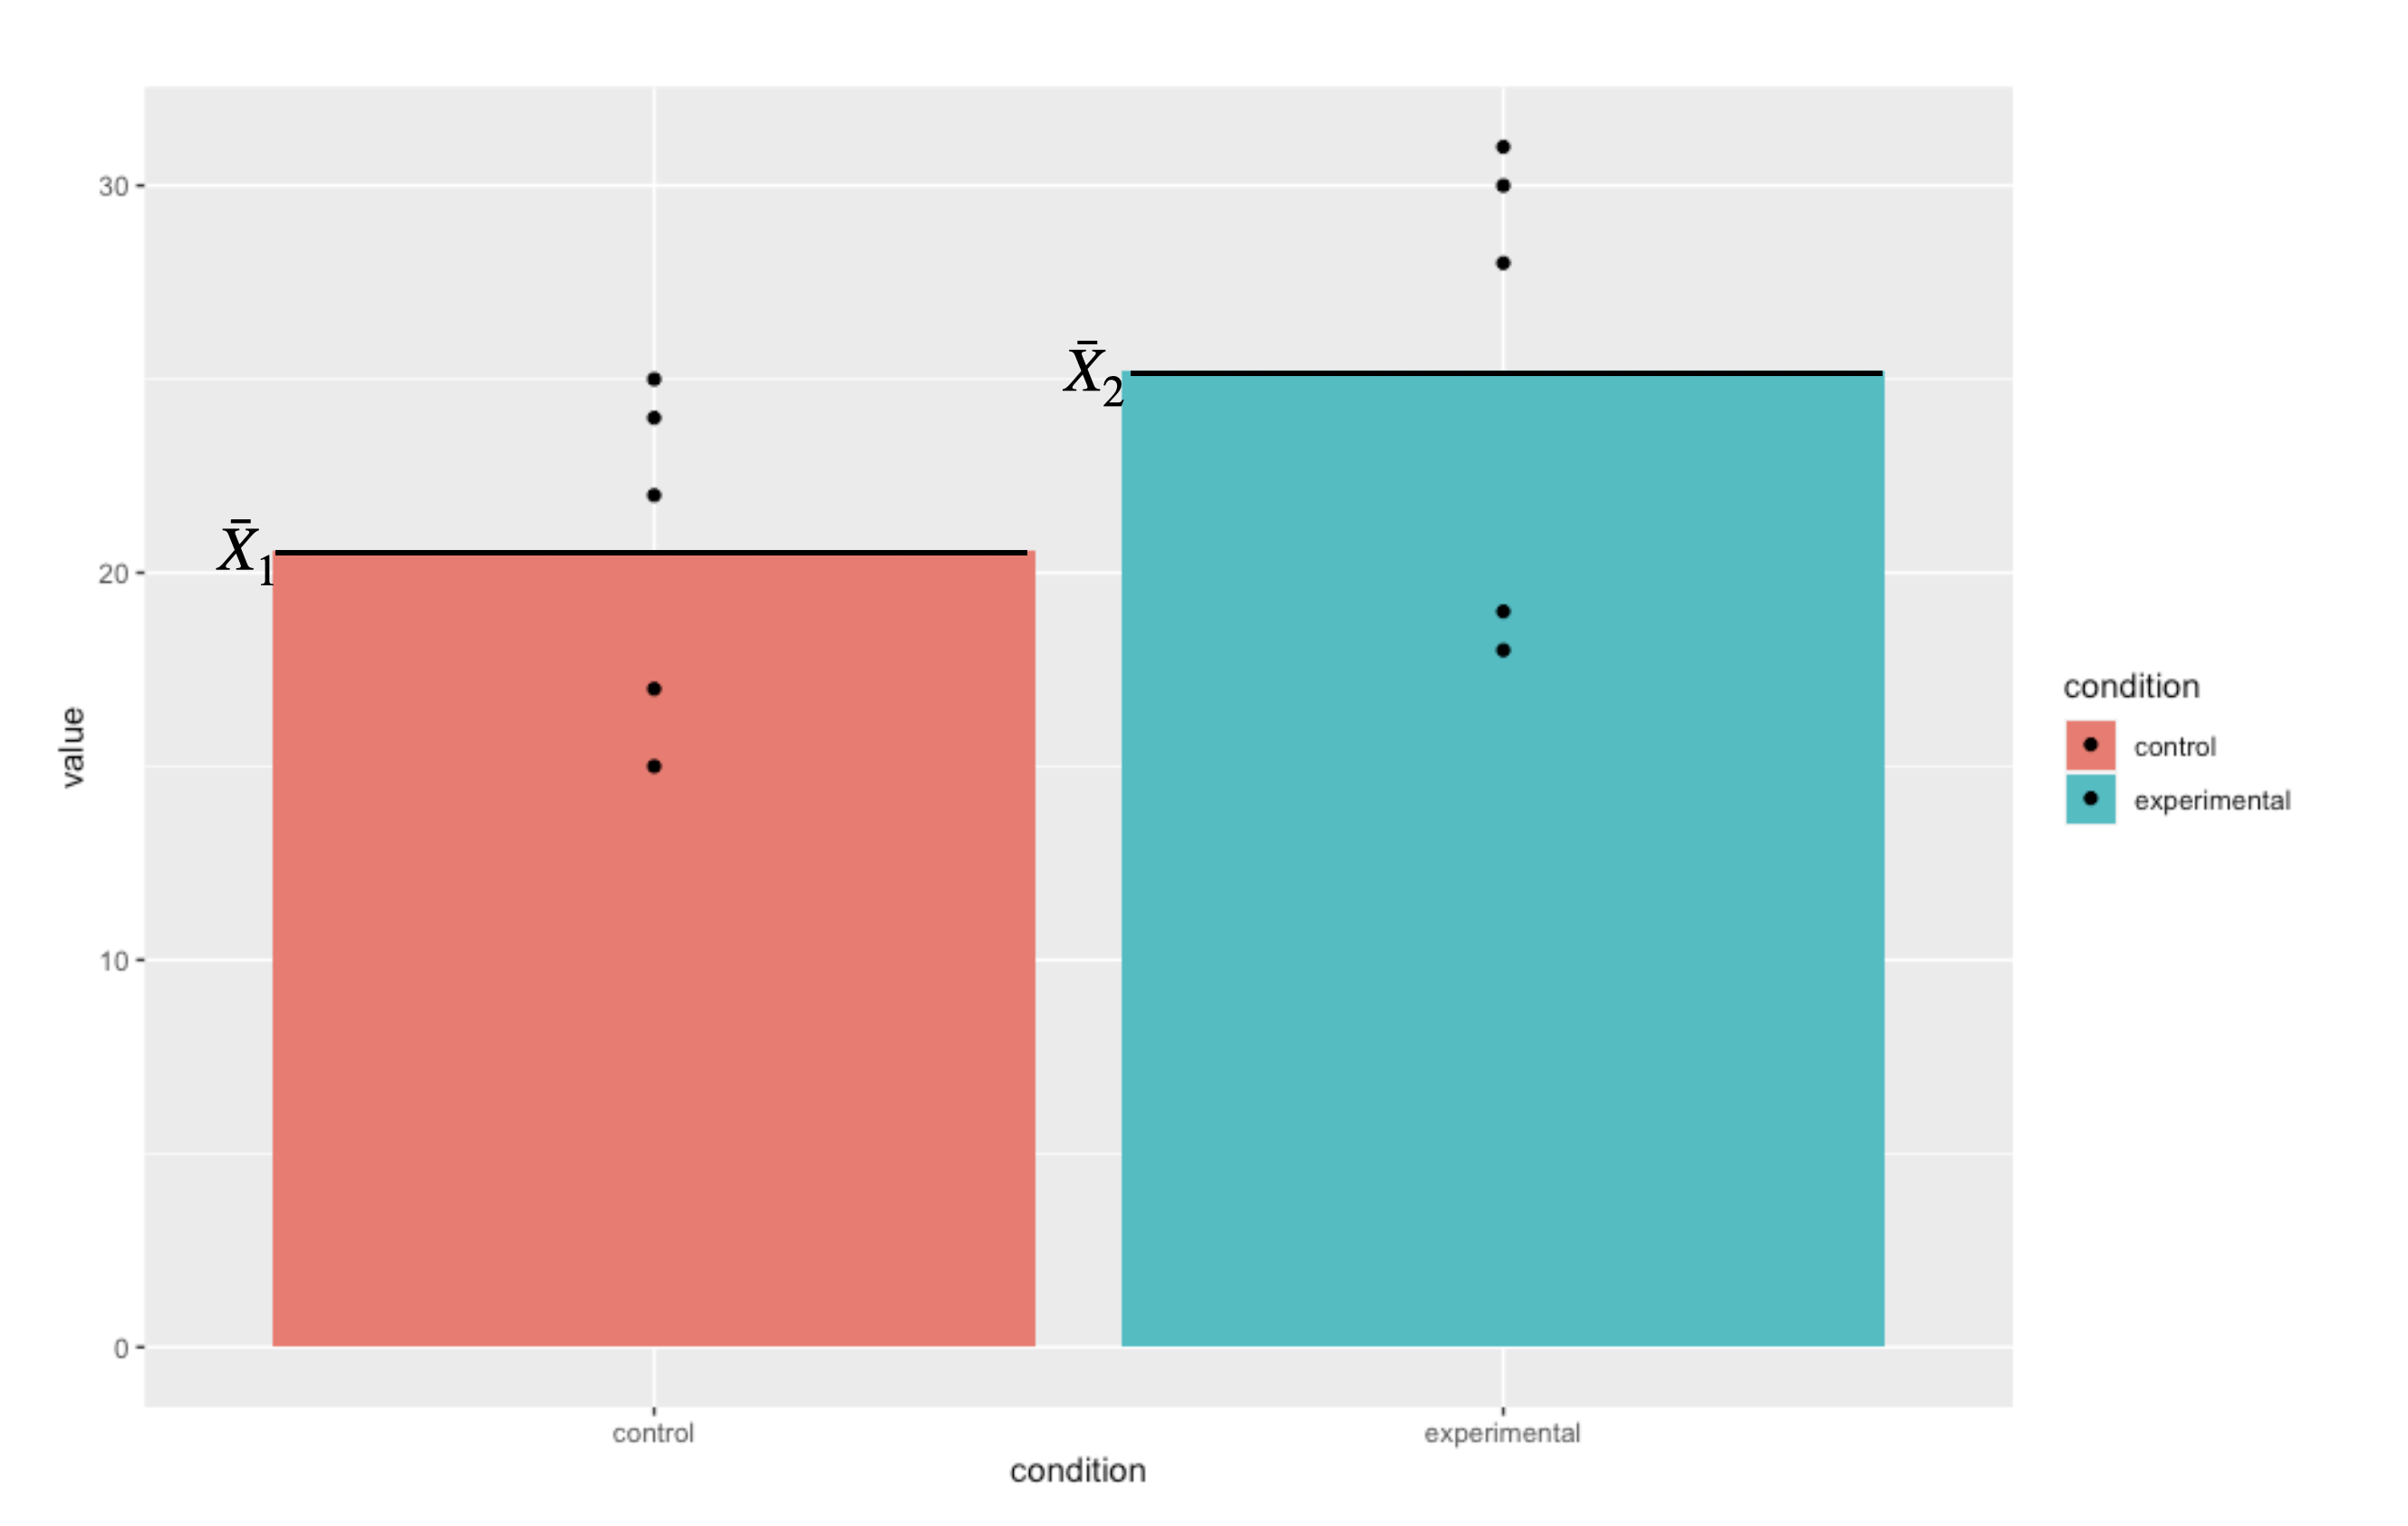
\includegraphics[keepaspectratio,width=8cm]{images/text21/slide21_01.png}
    \caption{2つの群の平均値のプロット。黒い点は各群のそれぞれの観測値}
    \label{fig::21_01}
\end{wrapfigure}

さて，最初に帰無仮説検定の話をしたときに，これはモデル比較だと言いました。帰無仮説というモデル，対立仮説というモデルを比較して，どちらに軍配を上げるかという勝負判定をする，これが帰無仮説検定だと。
ここでの「モデル」という言葉は，例えば帰無仮説は$\mu_1 - \mu_2 =0$をおく，といった表現がなされますから，前期の(線形)モデルという表現と異なるイメージを持ったかもしれません。しかしこれもモデル，しかも線形のモデルなのです。今からこの「帰無仮説検定」と「線形モデル」を概念的に統合することを説明してきます。

そのための例として，次のようなデータを用意しました(図\ref{fig::21_01})。これは対応のない，2つの群(仮に実験群と統制群とします)の平均値をプロットしたものです。ここで示されている平均値は標本平均ですから，そこに差があるのは見た通りです。ちなみに黒い点は各群における個体一つ一つの観測値です。

\subsection{平均値差の検定として考える}
まずは最近ずっと取り組んでいる，この標本平均から母平均を推測することを考えましょう。私たちは目の前のデータのこと「だけ」について考えているのではなく，議論を一般化したいのですから。母集団に正規分布を仮定すると，標本標準偏差や$t$分布を使って母平均を推測することができるのでしたね。

さて，ここで帰無仮説検定の，母平均に差がないと言うのはどういう状況でしょうか。$\mu_1 - \mu_2 =0$ というのはつまり，$\mu_1 = \mu=2$と言うことと同じですから，同じ平均値を持つ正規分布からデータが得られたと仮定した，と言うことになります(図\ref{fig::21_04})\footnote{特に$t$検定においては標準偏差も同じと仮定しますから，同一の正規分布になります}。
\begin{figure}[ht]
    \centering
    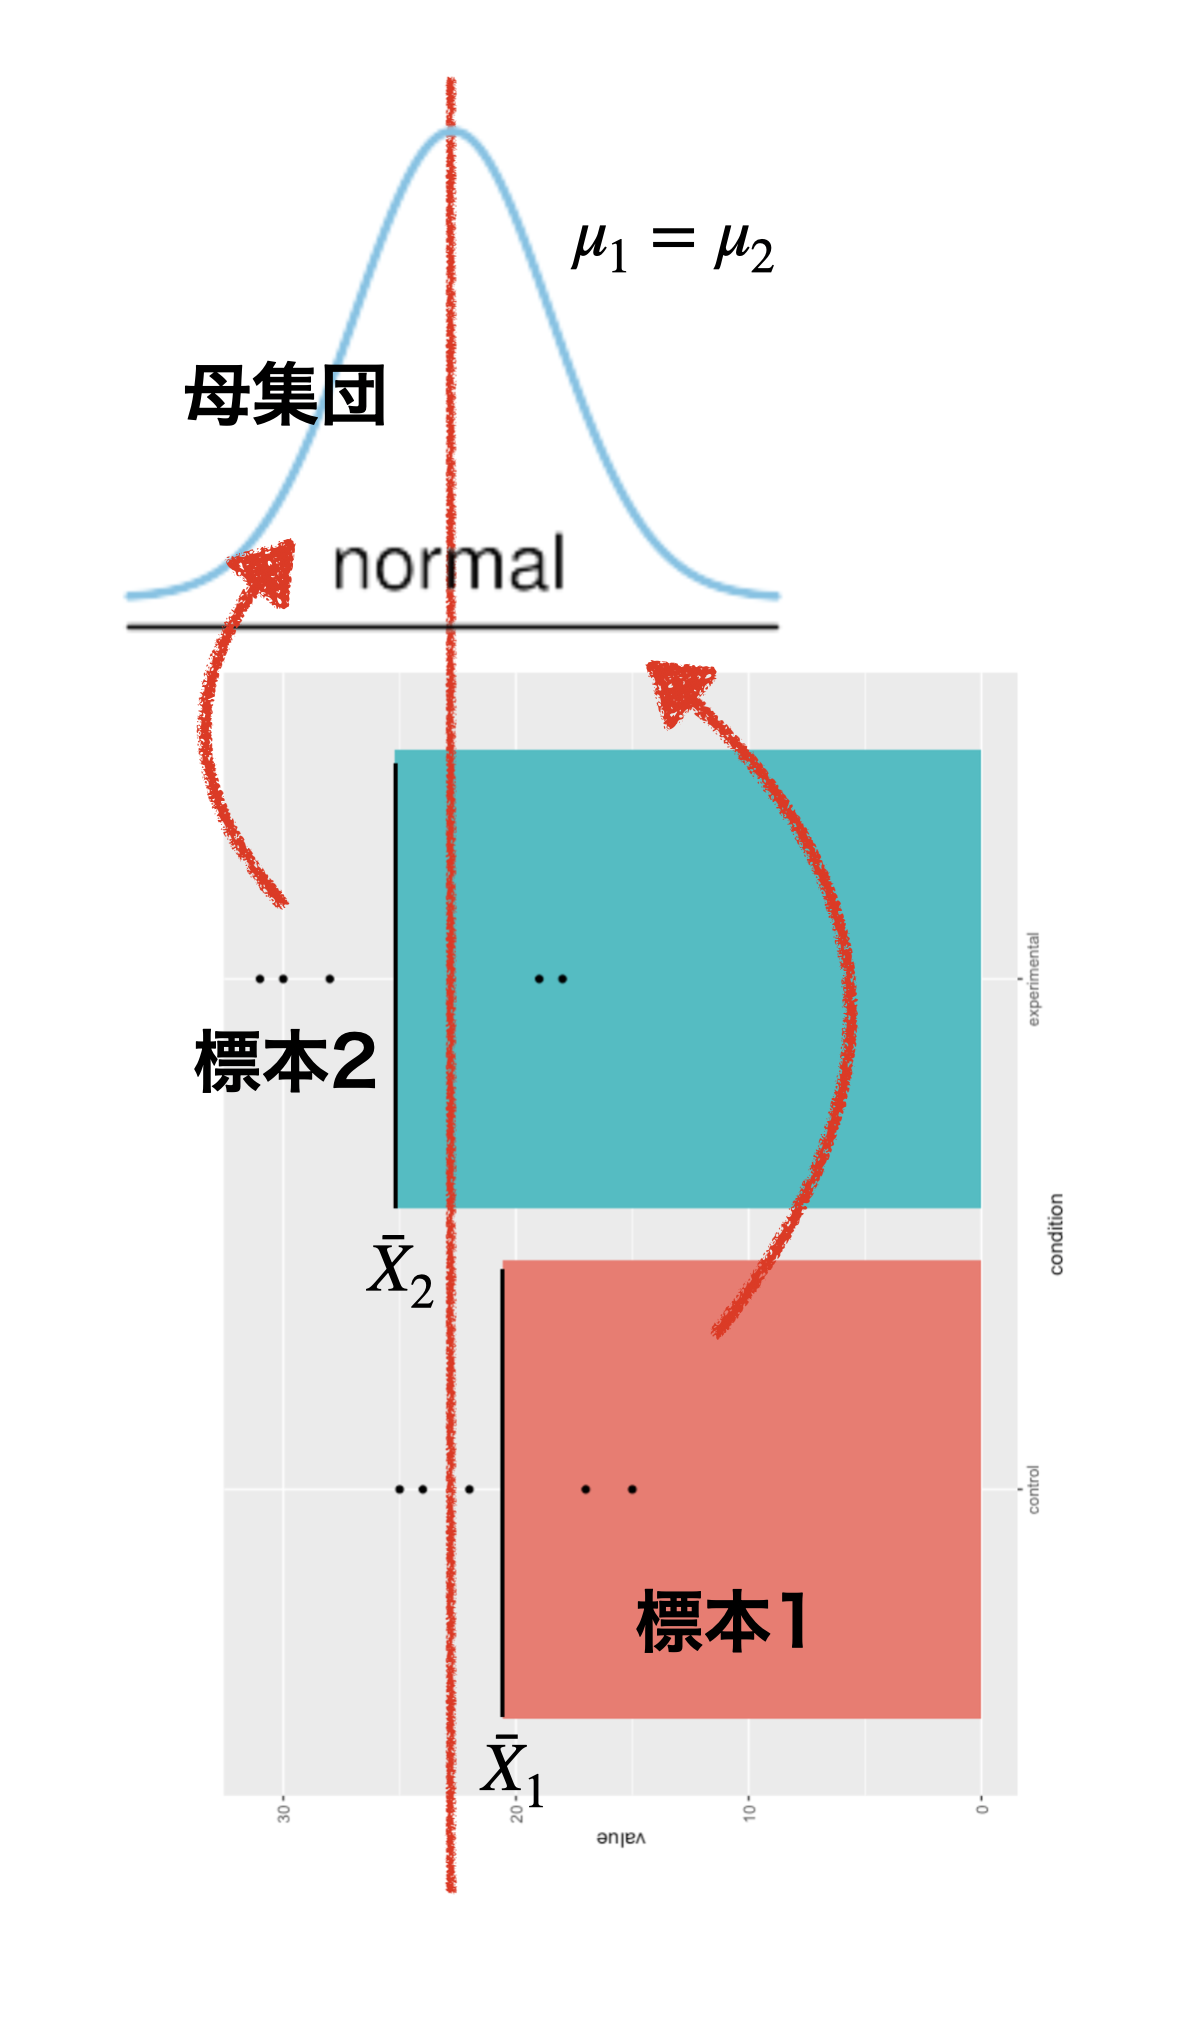
\includegraphics[keepaspectratio,width=8cm]{images/text21/slide21_04.png}
    \caption{母集団が上になるように元の図を回転しています}
    \label{fig::21_04}
\end{figure}

それぞれの標本平均から推定される，母平均の位置は幅を持って推定されますから，その幅がどの程度重複しているのかを考える必要があります。同じだと言えるほど重複しているのか，イエスかノーか，と差し迫った状況では何らかの基準を持って決めないといけませんから，間違って差があると言ってしまう可能性を低く抑えつつ(有意水準$\alpha=0.05$にするのが一般的)，結論を出しましょうというのが帰無仮説検定でしたね。

\subsection{神様の目から見た実験計画}
ここで，同じデータを別の見方で捉えてみましょう。

今回の例において，従属変数である心理変数はどう言う特徴なのか，目に見えないものなのでわかりません。でも，心の問題は無数の要因が積み重なった結果であると考えると，正規分布を仮定するのが自然です。つまり，実験群のひとも統制群のひとも，大きな視点から考えれば同じ人間という正規母集団からのサンプルなのです。

さて，実験参加者たちは実験者によって無作為に実験群と統制群に割り当てられました(RCT)。個人差がなければ，各群1名ずつのスコアを比較して考えれば良いのですが，人間を対象にしている以上そうはいきません。個人差がどうしても生じてしまうので，複数人を集めて個人差を相殺することを考えます。各群の平均値の違いを見ることで，操作の効果を見ることにするのです。

もしこの実験に効果がなければ，2群の平均値は同じになるでしょう。この時の平均値は，実験群と統制群に分けた効果がないのですから，両群のスコアを足しあわせた全体平均になるはずです。効果がない=全体平均，なのです。しかし，群ごとに見てみると全体平均から違いが生じています。図\ref{fig::21_03}では，統制群は相対的に低く，実験群は相対的に高い平均値を示しています。この差分こそ(図\ref{fig::21_03}では短い緑の矢印で示しています)，実験の効果なのです。

\begin{figure}[hb]
    \centering
    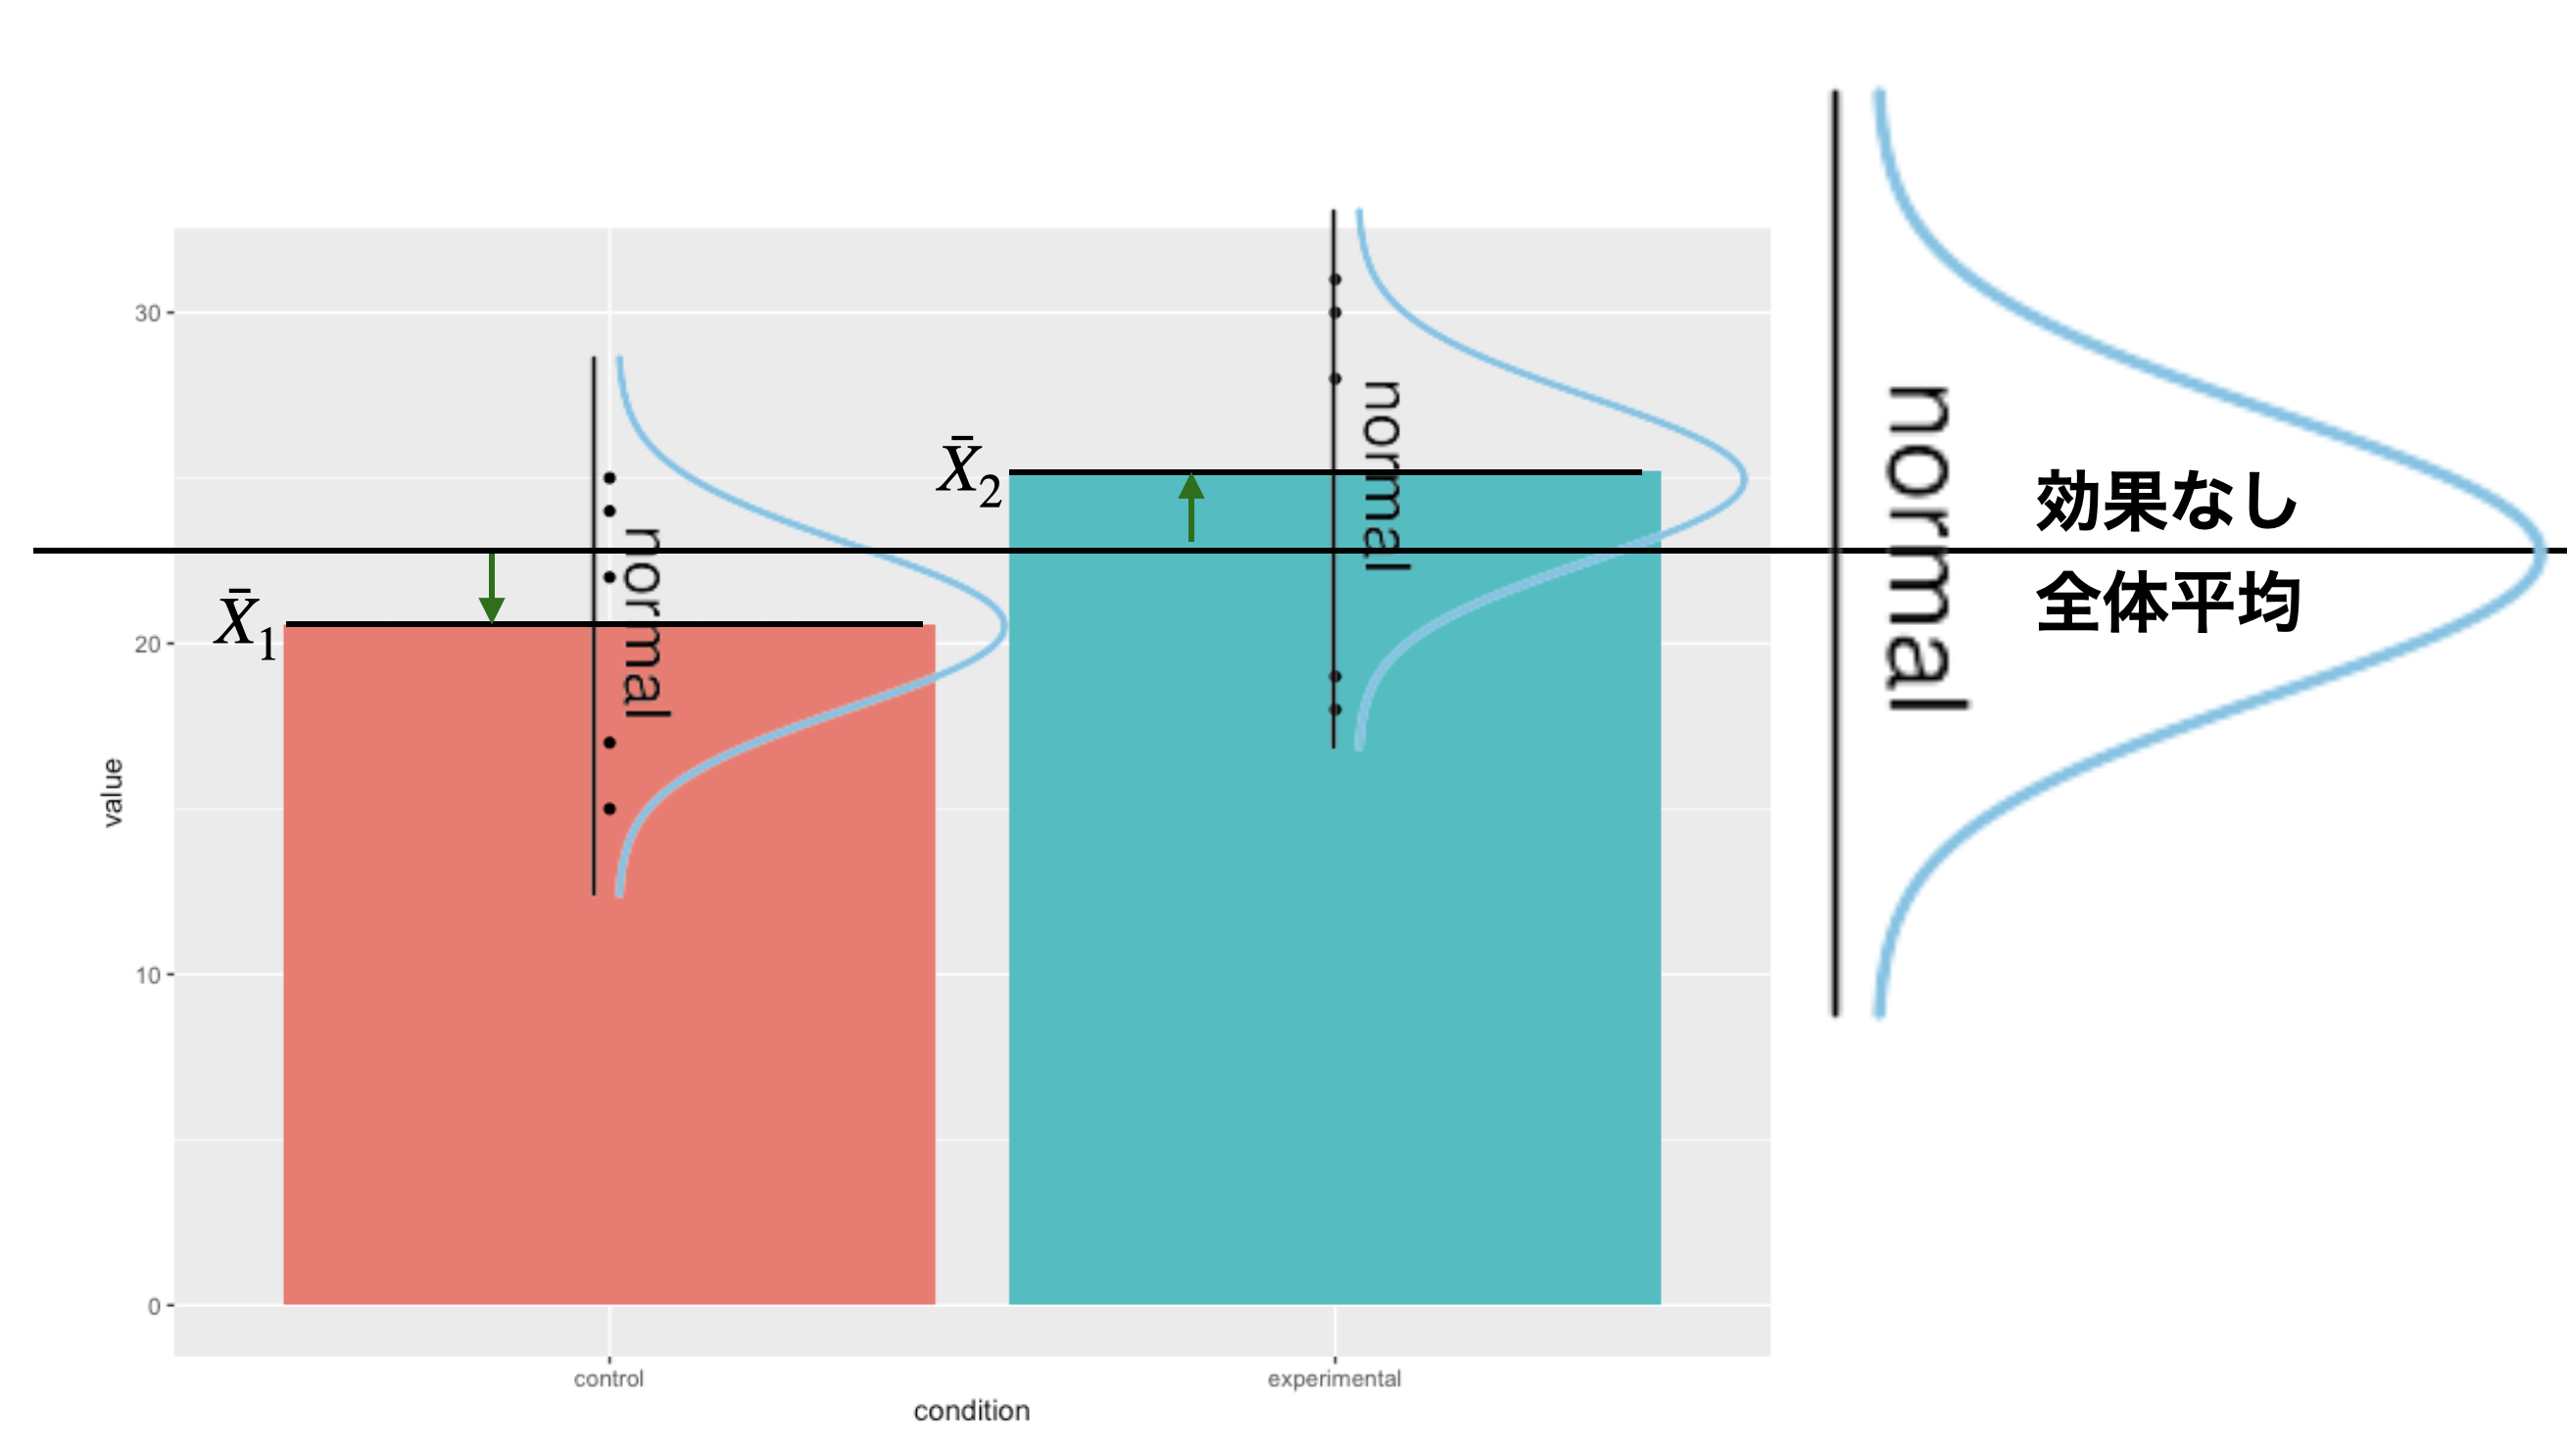
\includegraphics[keepaspectratio,width=12cm]{images/text21/slide21_03.png}
    \caption{効果がなければ全体平均に同じ。群の効果は相対的に平均値をずらす。}
    \label{fig::21_03}
\end{figure}

このことを，数式的な表現で考えてみたいと思います。
まず，各群のデータを$X_{ij}$で表します。ここで$i$は実験参加者の番号，$j$は実験群か統制群かを表す記号だと思ってください。仮想データとの対応を表\ref{tbl::21_01}に示しておきます\footnote{ここでのデータは第\ref{chapter19},\ref{chapter20}講の一要因群間2水準の$t$検定データと同じで，表は\ref{tbl::19_02}に少し手を加えたものです。手を加えた部分は，数式表現の列(notation)はもちろんなのですが，IDのところを通し番号から群ごとの番号に変えました。こうすることで，各群$N=5$だな，ということがわかりやすくなったかと思います。}。

\begin{table}[ht]
    \centering
    \caption{仮想データ例と記号の対応} 
    \begin{tabular}{rlcr}
      \hline
    ID & condition & notation & value \\ 
      \hline
    1 & control & $X_{11}$ & 25 \\ 
      2 & control & $X_{21}$& 15 \\ 
      3 & control & $X_{31}$& 24 \\ 
      4 & control & $X_{41}$& 17 \\ 
      5 & control &  $X_{51}$&22 \\ 
      1 & experimental & $X_{12}$& 31 \\ 
      2 & experimental & $X_{22}$& 28 \\ 
      3 & experimental & $X_{32}$& 30 \\ 
      4 & experimental & $X_{42}$& 19 \\ 
      5 & experimental & $X_{52}$& 18 \\ 
       \hline
    \end{tabular}
    \label{tbl::21_01}
\end{table}

さて，群ごとの平均は次のように書くことができます。
$$ \bar{X}_1 =\frac{1}{5} \sum_{i=1}^5 X_{i1} $$
$$ \bar{X}_2 =\frac{1}{5} \sum_{i=1}^5 X_{i2} $$
また，全体平均を次のように書くことができます\footnote{gmはgrand meanの略です。}。
$$ \bar{X}_{gm} = \frac{1}{10} \sum_{i} \sum_{j} X_{ij} $$
ここで群わけの効果が$\delta$だとすると\footnote{$\delta$はギリシア文字で「デルタ」の小文字です。ちなみに大文字は$\Delta$です。}
$$ \bar{X}_1 = \bar{X}_{gm} - \delta $$
$$ \bar{X}_2 = \bar{X}_{gm} + \delta $$
ということになります。

ここで，個人差はこの実験で制御できない誤差であり，群平均を中心にどういう向きで出るかわからないものですから，このことを表現するなら，
$$ X_{ij} = \bar{X}_j + \epsilon_{ij} $$
ということになります。これらを組み合わせると，
$$ X_{i1} = \bar{X}_{gm} - \delta + \epsilon_{i1} $$
$$ X_{i2} = \bar{X}_{gm} + \delta + \epsilon_{i2} $$
と書くことができます。ここで一工夫。$\delta$にプラス，マイナスの符号がついているのは，$+1,-1$を掛け算していると考えてみましょう。この符号を決めているものを$\beta_{11}=+1,\beta_{12}=-1$と表したとすると，まとめて次のように書くことができます。
\begin{equation}
    \label{eq::21_1}
     X_{ij} = \bar{X}_{gm} + \beta_{1j} \delta + \epsilon_{ij} 
\end{equation}
これ，どこかで見覚えありませんか。そうです，前期の間にやった回帰分析と同じ形をしているのです($\to$第\ref{chapter8}講参照)。

回帰分析を今ここで大雑把に復讐しておきますと，二つの変数$x_i,y_i$があったときに，両者の間に何らかの関数関係がある，と考えましょうという話でした。関数関係とは，一方を定めれば他方も定まるという関係ですから，この関係を数式で表現してやれば予測もできるぞ，嬉しいぞ。ということで，最も簡単な関数関係って何だ？そう，中学校の時にやった一次関数$y=ax+b$だよね，ということでした。ただ中学校の時の話とは違って，データがたくさんあり，かつ，全部にぴったり当てはまる線は引けない。なので，ちょっと誤差はあるけどだいたいあってる線を引こうね，ということを考えたのでした。この関数(一次関数，線形関数，線形モデル)で予測される値を$\hat{y}_i$と表したとすると,

$$ \hat{y}_i = b_0 + b_1x_i $$
データ$y_i$は予測値$\hat{y}_i$に誤差$e_i$がついて現れるから，
$$ y_i = \hat{y}_i + e_i $$
なので，これを統合して
$$ y_i = b_0 + b_1 x_i + e_i $$
としたのでした。

さてさて。記号で$y_i,x_i$とか$b_0,b_1$だったのが$X_{ij}$とか$\beta_{ij}$などと変わってはいますが，基本的には$y=ax+b$の一次線形関数の形です(図\ref{fig::21_05})。
\begin{figure}[ht]
    \centering
    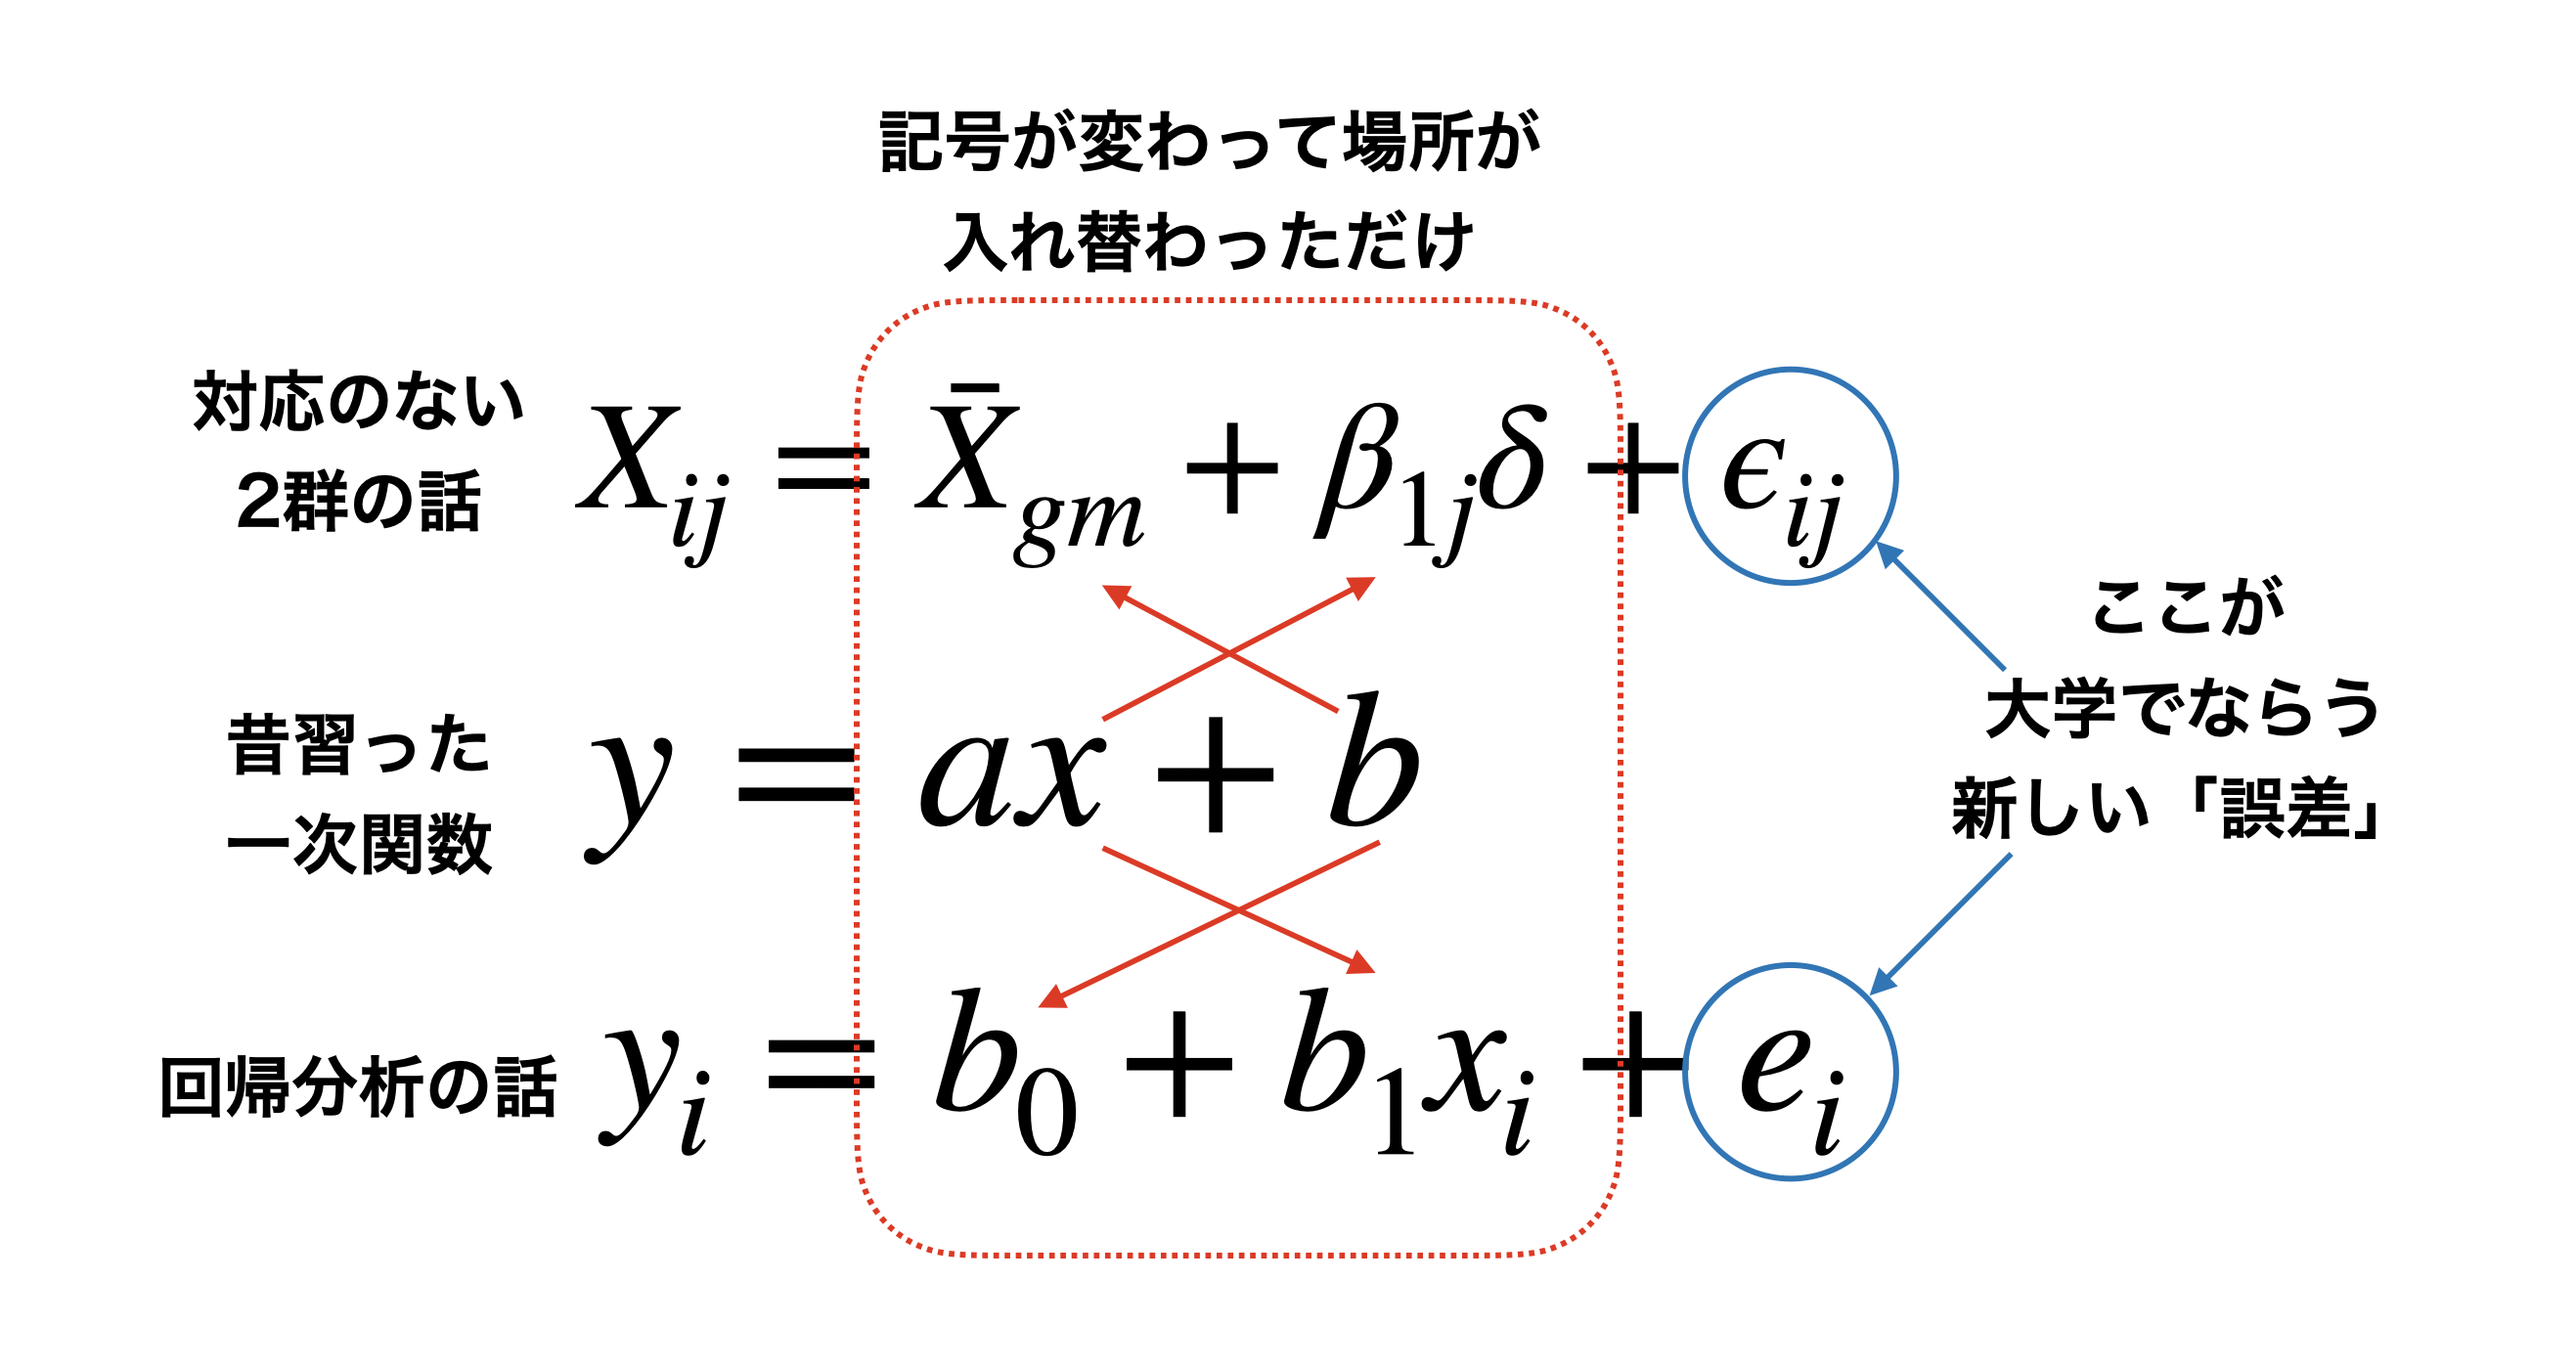
\includegraphics[keepaspectratio,width=12cm]{images/text21/slide21_05.png}
    \caption{数学的には記号が変わっても使われ方が同じであれば同型と考えます}
    \label{fig::21_05}
\end{figure}


先ほど，効果がない＝全体平均，という言い方をしました。効果のことを，記号$\delta$で表しているのですから，効果がないというのは$\delta=0$ということです。そうすると$\beta_1$ の項が消えてしまいます。つまり，全体平均$\bar{X}_{gm}$に誤差$\epsilon_{ij}$がついただけで，データは一つの正規分布から出てきたまま，ということになります。

一つの共通の正規分布。2つの群に分かれない，同じ正規分布。そろそろ帰無仮説検定と繋がってきたのではないでしょうか。効果がない，というのはまさに，帰無仮説のことですよね。つまり帰無仮説は，$\delta=0$という傾きゼロの直線，図\ref{fig::21_03}では群平均を横切っている，横一線の線形モデルだったのです。平均値の差の検定というのは，群平均が横一直線＝傾きゼロではないよ，という結論を出すためのロジックであり，比較される対立仮説は「傾きゼロでない何か」というモデルです。繰り返しになりますが，帰無仮説が傾きゼロという一点ばりに対し，対立仮説はゼロ以外であれば何でも良いという非常に非対称な戦いであり，結論が出たからと言って「じゃあゼロでない，何なのか」ということまでは強く主張できません。帰無仮説検定は補助的に使いつつ，実質はどのように傾いているのか，差の信頼区間はどの程度あるのか，効果量(標準化された平均値の差)は大きいのかといった，実質的な大きさを考えることが重要です。

ところでこの話は，第\ref{chapter11}講「回帰分析の特別な場合」として，既に紹介してあったものです。回帰分析では説明変数も従属変数も連続変数である，ということでしたが，説明変数が離散的になれば回帰線は両群の平均を通り(資料\ref{fig::ch11B_51} から\ref{fig::ch11B_61}のあたり)，傾きが平均の差である，という話をしました。その時は切片が一方の群平均にありましたが，本質的には同じことです。

また，前期の回帰分析の時は最小二乗法を使って回帰係数を求めたのでした。ただ，その時は推測統計学的な発想を導入していませんでした。データに最もうまく適合するために計算すると，とにかく求められるよ，という説明の仕方だったかと思います。手元のデータの話，つまり標本の話しかしていませんでしたので，係数として$b_0,b_1$と書いていたのですが，推測統計学の枠組みでこれを考えると，我々が知りたいのは母集団における傾き，母数だということになりますので，今回ギリシア文字$\beta_1$とか$\epsilon_{ij}$としたのです\footnote{スライドを見返すと，第\ref{chapter11}講では$\beta_0,\beta_1$で書いてました。すみません。}。うふふ。

平均値差の検定と回帰分析は同じものなのだ，という話をしてきました。いずれも正規分布を仮定しており，その意味が「心理現象に仮定される全体傾向をあらわす分布」なのか「誤差の分布」なのか，という微妙な出自の違いを持っていると言えるかもしれません。しかし数学的には同じことなので，どちらの筋道からでも考えて，同じように利用することができます。

また，回帰分析の係数を最小二乗法で求めたように，推測統計の枠組みで平均値を推定するのに最小二乗法を使うのだろうか，と考えている人もいるかもしれません。実はこれが大変興味深いところなのですが，推測統計の枠組みでは正規分布という確率分布を利用しますから，誤差を最小にしようという解析的な(確率的でない，という意味でつかています)方法とは異なる考え方を使う必要があります。確率分布を使った母数の推定方法として，\keyterm{最尤法}と\keyterm{ベイズ法}という二種類の方法を今後説明していきますが，結論だけ先にいっておくと，幸いにして最小二乗法による答えと最尤法による答えは\textbf{ぴったり一致します}。

ちなみにこれまでやってきた，標本平均や標本分散から母数を推定する方法は，「モーメント法」というやり方に分類されます。何であれ，同じデータであれば推定値はだいたい同じになります。同じものを推定しようとしてるのですから，違ってきたらむしろ困りますわね。

\section{一要因Betweenデザイン，多水準の場合]}
\section{多重比較}
\section{分散分析表}
\section{二要因の場合}

\section{課題}


\end{document}
